\chapter{विषाणु-विज्ञान}\label{ch:b3:virology}

पृथ्वी पर कोई $10^{31}$ \omterm{def:b3:virology:virus}{विषाणु} कण हैं, यानी हर कोशिका पर दस, और समुद्र
में वे हर दिन सारे जीवाणुओं का पाँचवाँ भाग मार देते हैं। कोई \omterm{def:b3:virology:virus}{विषाणु}
कोशिका नहीं है: उसके पास न उपापचय है, न राइबोसोम, न स्वयं कुछ बनाने का
कोई उपाय। वह कोई जीनोम है --- दो जीन जितना छोटा, दो हज़ार जितना लंबा ---
जो किसी प्रोटीन खोल में लिपटा है, किसी कोशिका में घुसता है और कोशिका के
तंत्र को अपनी नकलें बनाने में लगा देता है। 1918 का इन्फ़्लुएंज़ा पाँच
करोड़ लोगों को ले गया; चेचक, जिसने अकेली बीसवीं सदी में तीस करोड़ लोग
मारे, 1980 में उस टीके से समाप्त कर दी गई जो पहली बार 1796 में आज़माया
गया था; और 2019 में मनुष्यों में आए किसी कोरोना \omterm{def:b3:virology:virus}{विषाणु} का जीनोम हफ़्तों
में अनुक्रमित हुआ, उसके दिनों के भीतर कोई \omterm{def:b3:virology:drugs}{टीका} अभिकल्पित हुआ, और दो
वर्षों में उसके प्रोटिएज़ के विरुद्ध औषधें। यह अध्याय बताता है कि
\omterm{def:b3:virology:virus}{विषाणु} क्या हैं और उनके जीनोमों की रसायन से उनका वर्गीकरण कैसे होता है,
वे कैसे बढ़ते हैं, किसी एक परपोषी के भीतर किसी संक्रमण की बलगतिकी ---
जिसे दो अवकल समीकरणों की एक जोड़ी इतनी अच्छी तरह बताती है कि उसने एड्स
का उपचार बदल दिया --- उनका विकास, और उनसे लड़ा कैसे जाता है।

\section{विषाणु क्या है}

\begin{definition}[विषाणु]\label{def:b3:virology:virus}
\index{विषाणु}\index{कैप्सिड}\index{परिवेष्टन}\index{विषाणुकण}\index{बाल्टिमोर वर्गीकरण}
कोई \emph{विषाणु} अनिवार्य अंतःकोशिकीय परजीवी है जिसमें कोई
न्यूक्लिक अम्ल जीनोम --- DNA या RNA, एकलड़ी या द्विलड़ी, रैखिक या
वलयाकार, एक अणु या कई --- किसी प्रोटीन \emph{कैप्सिड} में भरा होता है,
और अनेक स्थितियों में किसी परपोषी झिल्ली से लिए गए \emph{परिवेष्टन} में
लिपटा और विषाणुजन्य ग्लाइकोप्रोटीनों से जड़ा होता है। पूरा संक्रामक कण
\emph{विषाणुकण} है, जो अधिकांश के लिए \qtyrange{20}{300}{nm} चौड़ा होता
है (कुछ विशाल विषाणु एक माइक्रोमीटर तक पहुँचते हैं)। कैप्सिड एक या कुछ
प्रोटीनों की अनेक प्रतियों से बनते हैं जो कुंडलित सममिति (कोई छड़, जैसे
तंबाकू मोज़ेक विषाणु में) या बीसफलकी सममिति ($60T$ उपइकाइयों का कोई खोल,
$T = 1, 3, 4, 7,\dots$) में सजी होती हैं। \emph{बाल्टिमोर
वर्गीकरण} विषाणुओं को जीनोम से संदेशवाहक RNA तक के मार्ग से बाँटता है:
I, द्विलड़ी DNA (हर्पीज़, चेचक, ऐडिनोवायरस, अधिकांश फ़ेज); II,
एकलड़ी DNA (पार्वोवायरस); III, द्विलड़ी RNA (रोटावायरस);
IV, धन-लड़ी RNA, जो स्वयं संदेशवाहक है (पोलियो, हेपटाइटिस C, कोरोना
विषाणु); V, ऋण-लड़ी RNA, जो संदेशवाहक का पूरक है
(इन्फ़्लुएंज़ा, खसरा, रेबीज़, इबोला); VI, RNA जिसका प्रतिलोम अनुलेखन DNA
में होता है (रेट्रोवायरस, HIV); VII, DNA जिसकी प्रतिकृति किसी RNA
मध्यवर्ती से होती है (हेपटाइटिस B)। I को छोड़कर हर वर्ग को कोई ऐसा
एंज़ाइम लाना या बनाना पड़ता है जो कोशिका के पास नहीं --- कोई RNA-निर्भर
RNA पॉलीमरेज़, कोई प्रतिलोम अनुलेखक --- और वही एंज़ाइम अधिकांश
\omterm{def:b3:virology:drugs}{प्रति-विषाणु औषधों} के लक्ष्य हैं।
\end{definition}

\begin{proof}[प्रमाण-सामग्री]
इवानोव्स्की (1892) और बाइयेरिंक (1898) ने दिखाया कि तंबाकू का मोज़ेक रोग
ऐसे रस से संचरित होता है जो उन छन्नों से गुज़र जाता है जो सारे जीवाणु
रोक लेते हैं --- कोई \emph{contagium vivum fluidum}, यानी कोई जीवित
संक्रामक तरल। स्टैनली (1935) ने उस कारक, तंबाकू मोज़ेक \omterm{def:b3:virology:virus}{विषाणु}, को
क्रिस्टलित किया और दिखाया कि वह प्रोटीन है जिसमें (जैसा बॉडन और पिरी ने
पाया) \qty{5}{\%} RNA है। हर्षे और चेज़ (1952) ने किसी जीवाणुभोजी के
प्रोटीन को $^{35}$S से और उसके DNA को $^{32}$P से अंकित किया, उसे
\emph{E.~coli} को संक्रमित करने दिया, किसी मिश्रक में खाली खोल झाड़
दिए, और $^{32}$P कोशिकाओं के भीतर तथा $^{35}$S बाहर पाया: DNA घुसता है
और प्रोटीन पीछे रह जाता है, इसलिए निर्देश DNA ढोता है। फ़्रेंकेल-कोनराट
(1955) ने तंबाकू मोज़ेक \omterm{def:b3:virology:virus}{विषाणु} को प्रोटीन और RNA में अलग किया और एक
प्रजाति के RNA तथा दूसरी के प्रोटीन से संक्रामक कण फिर जोड़ दिए; संतति
RNA वाली प्रजाति की निकली।
\end{proof}

\begin{proposition}[आनुवंशिक मितव्ययिता: कैप्सिड सममित क्यों होते हैं]\label{prop:b3:virology:economy}
\index{आनुवंशिक मितव्ययिता}
किसी \omterm{def:b3:virology:virus}{कैप्सिड} को वह जीनोम घेरना पड़ता है जो उसका कूटलेखन करता है। द्रव्यमान
$m$ के किसी प्रोटीन को लगभग $m/\qty{110}{Da}$ कूटक चाहिए, यानी
$3m/110$ न्यूक्लियोटाइड, और RNA का वह खंड लगभग
$3m/110\times\qty{330}{Da} = 9m$ भारी होगा: कोई भी प्रोटीन अपने ही
द्रव्यमान से नौ गुना भारी न्यूक्लिक अम्ल से कूटबद्ध होता है। किसी
\emph{एक ही} प्रोटीन अणु से बना कोई खोल यदि किसी जीनोम को घेरे तो उसे
केवल अपना ही कूटलेखन करने के लिए अपने द्रव्यमान से नौ गुना भारी जीनोम
घेरना पड़ेगा, और कोई खोल जैविक घनत्व पर अपने द्रव्यमान से नौ गुना
न्यूक्लिक अम्ल रख नहीं सकता। निकास, जो क्रिक और वॉट्सन (1956) ने देखा,
यह है कि खोल किसी एक छोटे प्रोटीन की अनेक प्रतियों से बनाया जाए: तंबाकू
मोज़ेक \omterm{def:b3:virology:virus}{विषाणु} अपने \qty{6400}{nt} जीनोम के \qty{480}{nt} में
\qty{17.5}{kDa} का कोई आवरण-प्रोटीन कूटबद्ध करता है और उसकी $2130$
प्रतियाँ काम में लेता है। जो एक जैसी उपइकाइयाँ एक जैसे जमती हैं उन्हें
सममित रूप से सजाना पड़ता है, इसलिए \omterm{def:b3:virology:virus}{विषाणु} \omterm{def:b3:virology:virus}{कैप्सिड} या तो कुंडलियाँ हैं या
बीसफलक, और वही मितव्ययिता उन्हें स्वयं-संयोजन की क्षमता भी देती है,
क्योंकि हर उपइकाई को केवल अपने पड़ोसियों को पहचानना होता है।
\end{proposition}
\begin{proof}
द्रव्यमान-अनुपात इससे निकलता है कि कोई कूटक लगभग \qty{330}{Da} के तीन
न्यूक्लियोटाइड का है और कोई अवशेष लगभग \qty{110}{Da} का: $3\times 330/110 =
9$। \qty{40}{MDa} के किसी एक प्रोटीन का कोई \omterm{def:b3:virology:virus}{कैप्सिड} \qty{360}{MDa}
न्यूक्लिक अम्ल घेरता, यानी न्यूक्लिक-अम्ल घनत्व पर लगभग \qty{50}{nm}
त्रिज्या का कोई गोला, जबकि स्वयं प्रोटीन लगभग \qty{2}{nm} मोटाई और उसी
त्रिज्या का कोई खोल बनाता --- ज्यामितीय रूप से संभव है, पर
$360\,000$ अवशेषों का कोई एक पॉलिपेप्टाइड जो सही वलित हो, संभव नहीं, और
एक उत्परिवर्तन उसे नष्ट कर देता। $n$ एक जैसी उपइकाइयों के साथ
कूटलेखन की लागत $n$ गुना घट जाती है जबकि घिरा आयतन वही रहता है।
\end{proof}

\begin{omfigure}
\begin{tikzpicture}[every node/.style={font=\scriptsize}, >=stealth]
  \node[draw, thick, rounded corners, fill=omMeth!30, minimum width=2.4cm] (mrna) at (0,0) {mRNA $\to$ प्रोटीन};
  \node[draw, thick, rounded corners, fill=omDef!20, align=center] (I) at (-5.8,3.6) {I: dsDNA\\हर्पीज़, चेचक, फ़ेज T4};
  \node[draw, thick, rounded corners, fill=omDef!20, align=center] (II) at (-2.0,3.6) {II: ssDNA\\पार्वोवायरस};
  \node[draw, thick, rounded corners, fill=omThm!20, align=center] (III) at (2.0,3.6) {III: dsRNA\\रोटावायरस};
  \node[draw, thick, rounded corners, fill=omThm!20, align=center] (IV) at (5.8,3.6) {IV: (+)RNA\\पोलियो, हेपटाइटिस C,\\कोरोना विषाणु};
  \node[draw, thick, rounded corners, fill=omThm!20, align=center] (V) at (-5.6,-3.4) {V: ($-$)RNA\\इन्फ़्लुएंज़ा, खसरा,\\रेबीज़, इबोला};
  \node[draw, thick, rounded corners, fill=omProp!30, align=center] (VI) at (0,-3.4) {VI: RNA $\to$ DNA\\रेट्रोवायरस (HIV)};
  \node[draw, thick, rounded corners, fill=omProp!30, align=center] (VII) at (5.6,-3.4) {VII: RNA के ज़रिए DNA\\हेपटाइटिस B};
  \node[below, font=\tiny, align=center, gray!50!black] at (-5.8,2.9) {परपोषी RNA पॉलीमरेज़};
  \node[below, font=\tiny, align=center, gray!50!black] at (-2.0,3.05) {दूसरी लड़ी बनती है,\\फिर अनुलेखन};
  \node[below, font=\tiny, align=center, gray!50!black] at (2.0,3.05) {कण में विषाणुजन्य\\RNA पॉलीमरेज़};
  \node[below, font=\tiny, align=center, gray!50!black] at (5.8,2.75) {जीनोम ही mRNA है};
  \node[above, font=\tiny, align=center, gray!50!black] at (-5.6,-2.55) {विषाणुजन्य पॉलीमरेज़ उसकी नकल करती है};
  \node[above, font=\tiny, align=center, gray!50!black] at (0,-2.85) {प्रतिलोम अनुलेखक, समाकलन,\\फिर परपोषी पॉलीमरेज़};
  \node[above, font=\tiny, align=center, gray!50!black] at (5.6,-2.85) {DNA का अनुलेखन};
  \foreach \c in {I,II,III,IV,V,VI,VII} \draw[->, thick] (\c) -- (mrna);
\end{tikzpicture}

{\small बाल्टिमोर के सातों वर्ग, जीनोम से संदेशवाहक RNA तक के मार्ग से
छाँटे हुए। I को छोड़कर हर वर्ग को ऐसा एंज़ाइम चाहिए जो परपोषी कोशिका
नहीं देती --- किसी \omterm{def:b3:virology:drugs}{प्रति-विषाणु औषध} का स्वाभाविक लक्ष्य।}
\end{omfigure}

\begin{omfigure}
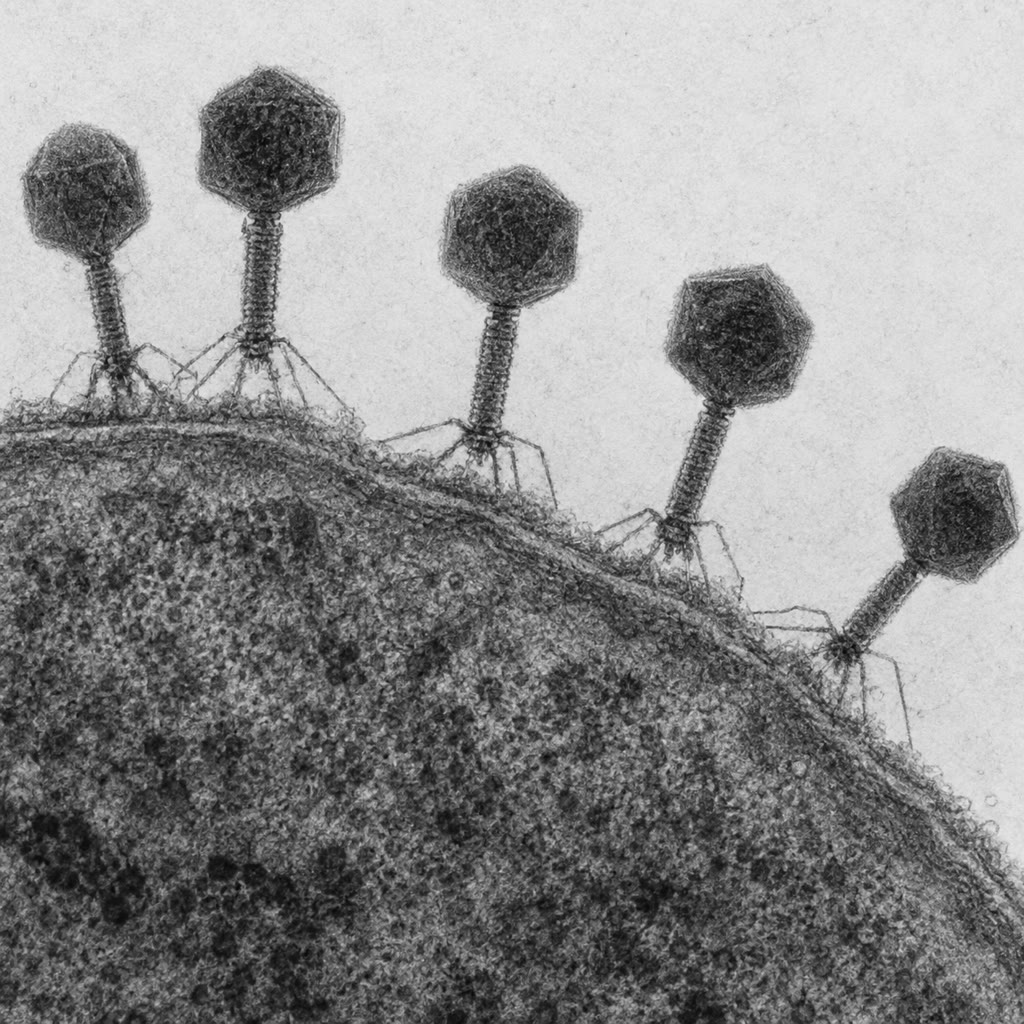
\includegraphics[width=0.36\linewidth]{images/book5/ai/b5-13-phage-tem.jpg}\hspace{0.04\linewidth}
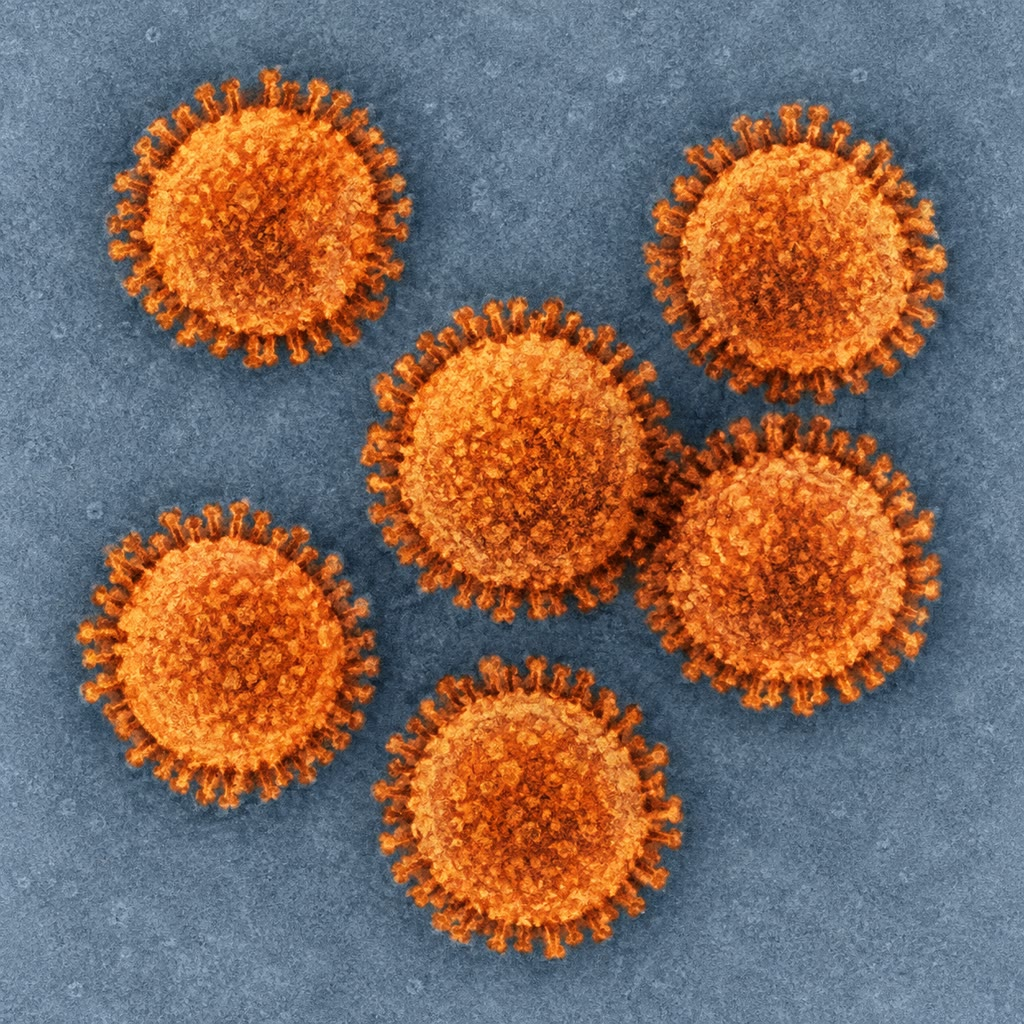
\includegraphics[width=0.36\linewidth]{images/book5/ai/b5-13-influenza-virions.jpg}

{\small बाएँ: किसी जीवाणु से अपने पुच्छ-तंतुओं से जुड़े जीवाणुभोजी,
जिनका हर सिर DNA का कोई बीसफलकी \omterm{def:b3:virology:virus}{कैप्सिड} है। दाएँ: इन्फ़्लुएंज़ा
\omterm{def:b3:virology:virus}{विषाणुकण}, परिवेष्टित, जिनका पृष्ठ हीमैग्लुटिनिन और न्यूरामिनिडेज़
काँटों की झालर है।}
\end{omfigure}

\section{कोई विषाणु कैसे बढ़ता है}

\begin{definition}[प्रतिकृति चक्र]\label{def:b3:virology:cycle}
\index{विषाणु प्रतिकृति चक्र}\index{ग्राही!विषाणुजन्य}\index{लयजनकता}\index{प्रसुप्ति}
हर \omterm{def:b3:virology:virus}{विषाणु} उन्हीं चरणों से गुज़रता है। किसी विशिष्ट परपोषी ग्राही से
\emph{जुड़ाव} --- HIV के लिए CD4 और कोई कीमोकाइन ग्राही, SARS कोरोना
\omterm{def:b3:virology:virus}{विषाणुओं} के लिए ACE2, इन्फ़्लुएंज़ा के लिए सियालिक अम्ल, किसी फ़ेज के
लिए कोई \omterm{def:b3:bacteriology:envelope}{लिपोपॉलिसैकेराइड} या कोई पोरिन --- जो तय करता है कि \omterm{def:b3:virology:virus}{विषाणु} किन
जातियों और किन कोशिकाओं को संक्रमित कर सकता है (उसकी \emph{परपोषी-रुचि})।
\emph{प्रवेश}: \omterm{def:b3:virology:virus}{परिवेष्टन} का जीवद्रव्य-कला से संलयन, या अंतर्ग्रहण और
उसके बाद अम्लीय \omterm{def:b3:membrane-traffic:endocytosis}{अंतःकाय} के भीतर से संलयन, या, किसी फ़ेज के लिए, दीवार
के पार जीनोम का अंतःक्षेपण। \emph{अनावरण}, वर्ग-विशिष्ट मार्ग से
विषाणुजन्य जीनों की \emph{अभिव्यक्ति}, और जीनोम की \emph{प्रतिकृति}, जो
प्रायः किसी ऐसी कारख़ाने में होती है जो \omterm{def:b3:virology:virus}{विषाणु} कोशिकाद्रव्य या केंद्रक
में बना लेता है। नए जीनोमों के चारों ओर नए \omterm{def:b3:virology:virus}{कैप्सिडों} का \emph{संयोजन},
जिसे सममित उपइकाइयों का स्वयं-संयोजन चलाता है, और \emph{मोचन}:
कोशिका के लयन से, या किसी झिल्ली से मुकुलन द्वारा, जो \omterm{def:b3:virology:virus}{परिवेष्टन} देता
है। कुछ \omterm{def:b3:virology:virus}{विषाणु} इसके बजाय अपना जीनोम परपोषी के जीनोम में डालकर प्रतीक्षा
कर सकते हैं: फ़ेज $\lambda$ की \emph{लयजनकता}, जिसका दमनकारी उसे तब तक
चुप रखता है जब तक परपोषी क्षतिग्रस्त न हो; हर्पीज़ \omterm{def:b3:virology:virus}{विषाणुओं} की
न्यूरॉनों में जीवन भर की \emph{प्रसुप्ति} और HIV की शांत T~कोशिकाओं में
किसी प्रोविषाणु के रूप में, जहाँ से उसे प्रतिकृति पर काम करती कोई भी
औषध नहीं हटाती।
\end{definition}

\begin{omfigure}
\begin{tikzpicture}[every node/.style={font=\scriptsize}, >=stealth]
  % cell
  \draw[very thick, omDef, fill=omDef!6] (0,0) ellipse (5.6 and 3.2);
  \draw[thick, omDef!70, fill=omDef!20] (1.8,0) ellipse (1.6 and 1.1); \node at (1.8,0.75) {केंद्रक};
  % virion outside
  \draw[thick, omProp, fill=omProp!30] (-7.2,1.6) circle (0.35); \foreach \a in {0,45,...,315} \draw[omProp, thick] (-7.2,1.6) ++(\a:0.35) -- ++(\a:0.15);
  \node[above] at (-7.2,2.1) {विषाणुकण};
  \draw[->, thick] (-6.8,1.4) -- (-5.7,0.9); \node[below, align=center] at (-6.6,1.0) {1. ग्राही से\\जुड़ाव};
  % entry
  \draw[thick, omProp] (-5.4,0.7) arc[start angle=140, end angle=40, radius=0.5];
  \node[below, align=center] at (-3.9,-0.2) {2. संलयन या अंतर्ग्रहण;\\3. अनावरण};
  % genome path
  \draw[omThm, very thick] (-3.4,0.2) .. controls (-2.6,0.6) .. (-1.8,0.4);
  \draw[->, thick] (-1.6,0.4) -- (-0.4,0.4);
  \node[above, align=center] at (-1.0,0.55) {4. जीन अभिव्यक्ति,\\जीनोम प्रतिकृति};
  \draw[omThm, very thick] (-1.0,-0.5) -- (0.4,-0.5); \draw[omThm, very thick] (-1.0,-0.75) -- (0.4,-0.75); \draw[omThm, very thick] (-1.0,-1.0) -- (0.4,-1.0);
  % assembly
  \foreach \p in {(1.2,-1.6),(1.9,-1.9),(2.6,-1.5)} { \draw[thick, omProp, fill=omProp!30] \p circle (0.25); }
  \node[below, align=center] at (1.9,-2.2) {5. जीनोमों के चारों ओर\\कैप्सिड जुड़ते हैं};
  % budding
  \draw[thick, omProp, fill=omProp!30] (4.9,-1.7) circle (0.32); \draw[->, thick] (5.3,-1.75) -- (6.4,-2.0);
  \draw[thick, omProp, fill=omProp!30] (7.0,-2.2) circle (0.35); \foreach \a in {0,45,...,315} \draw[omProp, thick] (7.0,-2.2) ++(\a:0.35) -- ++(\a:0.15);
  \node[below, align=center] at (6.4,-2.6) {6. झिल्ली से मुकुलन\\(परिवेष्टन) या कोशिका का लयन};
  % latency
  \draw[->, thick, dashed, omMeth!70!black] (-0.2,0.2) -- (0.9,0.2); \node[below, omMeth!70!black, align=center, font=\tiny] at (2.0,-0.05) {रेट्रोवायरस: प्रोविषाणु\\के रूप में समाकलन; प्रसुप्ति};
\end{tikzpicture}

{\small किसी परिवेष्टित \omterm{def:b3:virology:virus}{विषाणु} का प्रतिकृति चक्र: किसी ग्राही से
जुड़ाव, प्रवेश और अनावरण, परपोषी के तंत्र में अभिव्यक्ति तथा प्रतिकृति,
संयोजन, और मुकुलन द्वारा मोचन --- या, किसी रेट्रोवायरस के लिए,
परपोषी जीनोम में समाकलन और चुप्पी।}
\end{omfigure}

\begin{method}[संक्रामक कण गिनना: पट्ट परीक्षण]\label{met:b3:virology:plaque}
\index{पट्ट परीक्षण}\index{अनुमापांक}
किसी \omterm{def:b3:virology:virus}{विषाणु} भंडार को मापने के लिए: (1) उसे दस-दस गुने चरणों में तनु
कीजिए; (2) हर तनुकरण को परपोषी कोशिकाओं की अधिकता से मिलाइए --- किसी
फ़ेज के लिए नरम ऐगार में जीवाणु, किसी प्राणी \omterm{def:b3:virology:virus}{विषाणु} के लिए संवर्धित
कोशिकाओं की कोई एकपरत; (3) उष्मायित कीजिए: हर संक्रामक कण एक कोशिका
संक्रमित करता है, संतति पड़ोसियों को संक्रमित करती है, और एक-दो दिन बाद
कोई स्वच्छ छेद, यानी कोई \emph{पट्ट}, उस स्थान को चिह्नित कर देता है;
(4) \numrange{30}{300} वाली किसी पट्टिका पर पट्ट गिनिए और तनुकरण से
गुणा कीजिए: यही प्रति मिलीलीटर पट्ट-निर्माणी इकाइयों (PFU) में
\emph{अनुमापांक} है। चूँकि हर पट्ट किसी एक कण का क्लोन है, उसे उठा लेने
से कोई शुद्ध निष्कर्ष मिल जाता है। भौतिक कणों (इलेक्ट्रॉन
सूक्ष्मदर्शिकी या PCR से गिने) और पट्ट-निर्माणी इकाइयों का अनुपात
प्रायः एक से कहीं ऊपर होता है --- अनेक प्राणी \omterm{def:b3:virology:virus}{विषाणुओं} के लिए दस से एक
हज़ार --- क्योंकि अधिकांश कण दोषपूर्ण होते हैं या संक्रमित नहीं कर पाते।
\end{method}

\begin{omfigure}
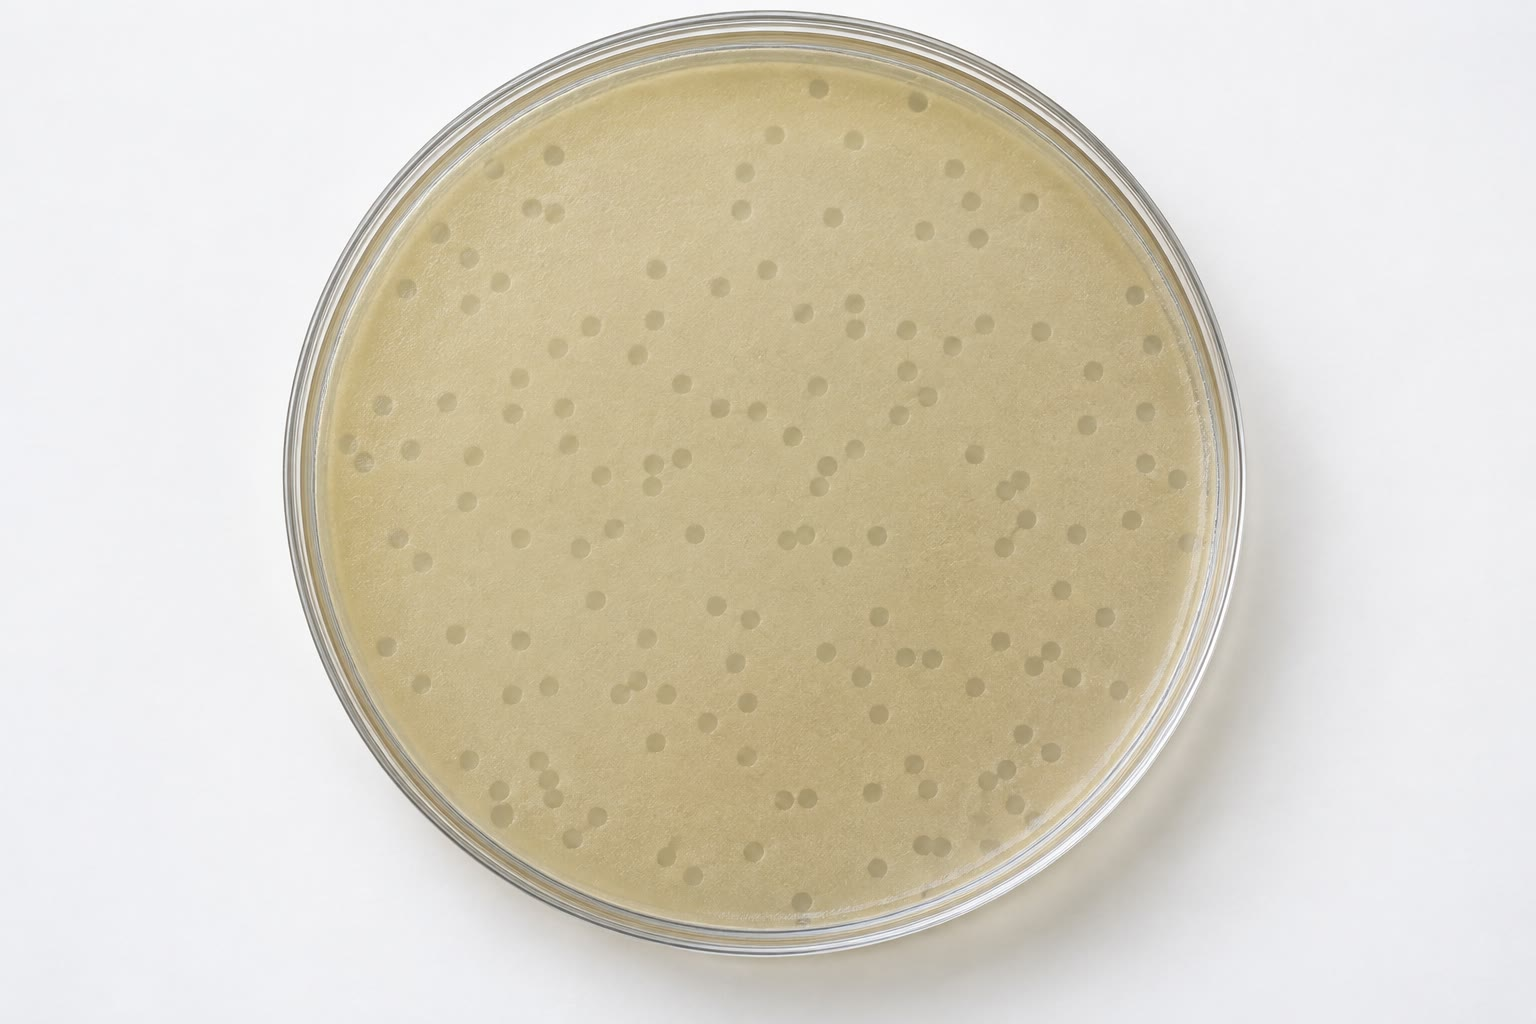
\includegraphics[width=0.46\linewidth]{images/book5/ai/b5-13-plaque-assay.jpg}\hspace{0.04\linewidth}
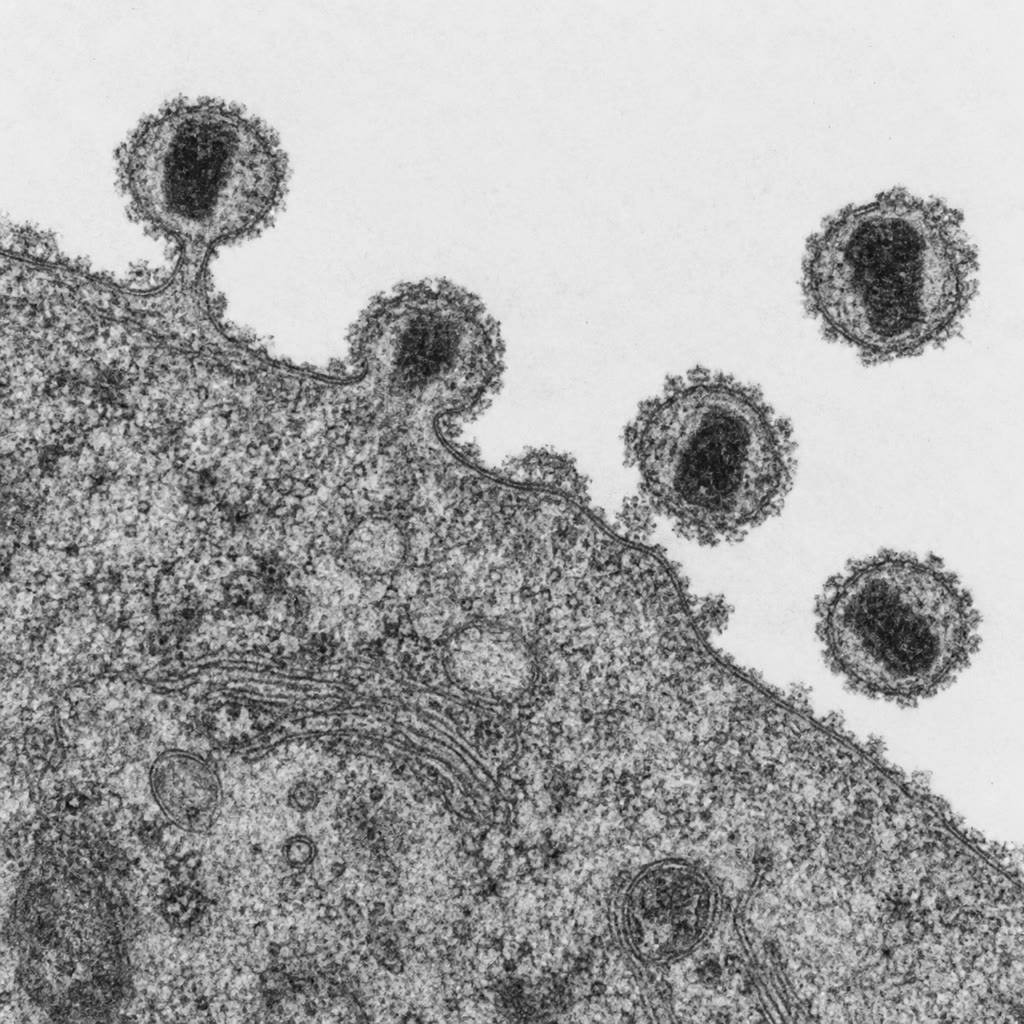
\includegraphics[width=0.36\linewidth]{images/book5/ai/b5-13-hiv-budding.jpg}

{\small बाएँ: किसी जीवाणु चादर में पट्ट, हर एक ऐसा स्वच्छ क्षेत्र जहाँ
किसी एक फ़ेज की संतति ने अपने चारों ओर की कोशिकाएँ लयित कर दी हैं।
दाएँ: किसी T~लसीकाणु से मुकुलित होते HIV कण, जो अपना \omterm{def:b3:virology:virus}{परिवेष्टन} कोशिका
की झिल्ली से ले रहे हैं।}
\end{omfigure}

\begin{theorem}[किसी परपोषी के भीतर संक्रमण की गतिकी]\label{thm:b3:virology:dynamics}
\index{मूल जनन संख्या!परपोषी-भीतर}\index{विषाणु-भार}\index{विषाणु गतिकी}
मान लीजिए $T$ संवेद्य लक्ष्य कोशिकाओं का घनत्व है, $I$ संक्रमित
कोशिकाओं का और $V$ मुक्त \omterm{def:b3:virology:virus}{विषाणुकणों} का। \omterm{def:b3:virology:virus}{विषाणुकण} लक्ष्यों को दर $\beta TV$
से संक्रमित करते हैं, संक्रमित कोशिकाएँ प्रति कोशिका दर $p$ से
\omterm{def:b3:virology:virus}{विषाणुकण} बनाती हैं और दर $\delta$ से मरती हैं, और मुक्त \omterm{def:b3:virology:virus}{विषाणुकण} दर
$c$ से साफ़ किए जाते हैं:
\[
\frac{\mathrm{d}I}{\mathrm{d}t} = \beta TV - \delta I, \qquad
\frac{\mathrm{d}V}{\mathrm{d}t} = pI - cV .
\]
$T$ को अचर मानें तो संक्रमण तब बढ़ता है जब \emph{मूल
जनन संख्या} $R_{0} = \beta Tp/(c\delta)$ $1$ से अधिक हो, और स्थायी
अवस्था पर $V^{*} = p I^{*}/c$ होता है, जिसमें उत्पादन सफ़ाई को संतुलित
करता है। यदि कोई औषध $t = 0$ पर सारे नए संक्रमण रोक दे ($\beta \to 0$),
तो \omterm{def:b3:virology:virus}{विषाणुकण} पहले सफ़ाई-दर $c$ से क्षीण होते हैं, फिर, जब मुक्त \omterm{def:b3:virology:virus}{विषाणु}
उस स्तर तक गिर जाए जिसे बची संक्रमित कोशिकाएँ बनाए रखती हैं, उन
कोशिकाओं की मृत्यु-दर $\delta$ से:
\[
V(t) \approx V_{0}\,\frac{c\,e^{-\delta t} - \delta\,e^{-ct}}{c - \delta}
\;\longrightarrow\; V_{0}\,\frac{c}{c-\delta}\,e^{-\delta t}
\quad (t \gg 1/c).
\]
उपचार के बाद \omterm{thm:b3:virology:dynamics}{विषाणु-भार} की दोनों ढालें $c$ और
$\delta$ मापती हैं, और $pI^{*} = cV^{*}$ उपचार से पहले \omterm{def:b3:virology:virus}{विषाणुकणों} का
दैनिक उत्पादन दे देता है।
\end{theorem}
\begin{proof}
कोई संक्रमित कोशिका औसतन $1/\delta$ जीती है और $p/\delta$
\omterm{def:b3:virology:virus}{विषाणुकण} बनाती है; हर \omterm{def:b3:virology:virus}{विषाणुकण} $1/c$ जीता है और उस समय में $\beta T/c$
कोशिकाएँ संक्रमित करता है; गुणनफल वह संख्या है जितनी संक्रमित कोशिकाएँ
एक संक्रमित कोशिका से बनती हैं, यानी $R_{0}$। स्थायी अवस्था पर
$\mathrm{d}V/\mathrm{d}t = 0$ से $V^{*} = pI^{*}/c$ मिलता है। उपचार के
बाद $\mathrm{d}I/\mathrm{d}t =
-\delta I$, इसलिए $I = I_{0}e^{-\delta t}$, और $\mathrm{d}V/\mathrm{d}t =
pI_{0}e^{-\delta t} - cV$ कोई रैखिक समीकरण है जिसका हल
$V(0) = V_{0} = pI_{0}/c$ के साथ वही व्यंजक है जो दिया गया है (जाँच: $t = 0$ पर
वह $V_{0}$ के बराबर है, और वह समीकरण को पद-दर-पद संतुष्ट करता है)। $t
\gg 1/c$ के लिए $e^{-ct}$ पद जा चुका होता है और $V$ ढाल $-\delta$ के
साथ संक्रमित कोशिकाओं का अनुसरण करता है; $t \ll 1/\delta$ और $c \gg \delta$
के लिए आरंभिक ढाल $-c$ है।
\end{proof}

\begin{example}[समीकरणों से पहले और बाद HIV]\label{ex:b3:virology:hiv}
1995 तक HIV संक्रमण की नैदानिक \omterm{def:b3:virology:cycle}{प्रसुप्ति} के वर्ष --- प्रति मिलीलीटर
$10^{4}$--$10^{6}$ प्रतियों का स्थिर \omterm{thm:b3:virology:dynamics}{विषाणु-भार} और T~कोशिकाओं की धीमी
गिरावट --- किसी शांत \omterm{def:b3:virology:virus}{विषाणु} के रूप में पढ़े जाते थे। हो, पेरेल्सन और
सहयोगियों ने रोगियों को कोई \omterm{def:b3:virology:drugs}{प्रोटिएज़ निरोधक} दिया और \omterm{thm:b3:virology:dynamics}{विषाणु-भार} की
गिरावट को प्रमेय से फिट किया: तेज़ प्रावस्था ने $c \approx \qty{3}{d^{-1}}$
दिया (किसी \omterm{def:b3:virology:virus}{विषाणुकण} का अर्ध-आयु काल लगभग छह घंटे), और धीमी प्रावस्था ने $\delta \approx
\qty{0.5}{d^{-1}}$ (कोई संक्रमित कोशिका लगभग डेढ़ दिन जीती है)। \qty{15}{L} शरीर-द्रव में प्रति मिलीलीटर $10^{5}$ का कोई
स्थिर भार, जो $c$ से साफ़ होता हो, इसलिए हर दिन, वर्षों तक, लगभग
$10^{10}$ \omterm{def:b3:virology:virus}{विषाणुकणों} का उत्पादन माँगता है: ``प्रसुप्त'' काल संक्रमण और
मृत्यु की कोई प्रचंड स्थायी अवस्था है, जिसमें T~कोशिकाओं का भंडार रोज़
बदला जाता है जब तक वह चुक न जाए। अगले खंड का उत्परिवर्तन-अंकगणित फिर
अपने आप निकल आता है, और उसके साथ यह कारण भी कि अकेली औषधें क्यों विफल
हुईं और तीन क्यों नहीं।
\end{example}

\begin{omfigure}
\begin{tikzpicture}
\begin{axis}[
  width=0.7\linewidth, height=5.8cm,
  axis x line=bottom, axis y line=left,
  xmin=0, xmax=14, ymin=10, ymax=2e5, ymode=log,
  xlabel={चिकित्सा शुरू करने के बाद के दिन}, ylabel={प्रति mL विषाणुकण},
  xlabel style={font=\small, at={(axis description cs:0.5,-0.12)}, anchor=north}, ylabel style={font=\small},
  tick label style={font=\small}, xtick={0,2,4,6,8,10,12,14},
  clip=false,
]
\addplot[very thick, omDef, domain=0:14, samples=100] {1e5*(3*exp(-0.5*x) - 0.5*exp(-3*x))/2.5};
\addplot[dashed, omThm, domain=0:1.6, samples=2] {1e5*exp(-3*x)};
\addplot[dashed, omMeth!70!black, domain=1.5:14, samples=2] {1e5*1.2*exp(-0.5*x)};
\node[font=\scriptsize, omThm, anchor=west] at (axis cs:1.8,600) {मुक्त विषाणुकण साफ़: ढाल $-c$, अर्ध-आयु \qty{6}{h}};
\node[font=\scriptsize, omMeth!70!black, anchor=south west] at (axis cs:5.5,1.5e4) {संक्रमित कोशिकाएँ मरती: ढाल $-\delta$, अर्ध-आयु \qty{1.4}{d}};
\end{axis}
\end{tikzpicture}

{\small किसी औषध द्वारा नए संक्रमण रोक देने के बाद \omterm{thm:b3:virology:dynamics}{विषाणु-भार}, प्रमेय
से, $c = \qty{3}{d^{-1}}$ और $\delta = \qty{0.5}{d^{-1}}$ के साथ: मुक्त
\omterm{def:b3:virology:virus}{विषाणुकणों} के साफ़ होते ही तेज़ गिरावट, फिर पहले से संक्रमित कोशिकाओं
की मृत्यु से तय धीमी गिरावट।}
\end{omfigure}

\section{विषाणु कैसे विकसित होते हैं}

\begin{definition}[उत्परिवर्तन, अर्ध-जाति, अपवाह और विस्थापन]\label{def:b3:virology:evolution}
\index{अर्ध-जाति}\index{प्रतिजनी अपवाह}\index{प्रतिजनी विस्थापन}\index{खंड-पुनर्मिश्रण}
RNA-निर्भर पॉलीमरेज़ों और प्रतिलोम अनुलेखकों में कोई शुद्धि-पाठन नहीं
होता, और RNA \omterm{def:b3:virology:virus}{विषाणु} प्रति न्यूक्लियोटाइड प्रति प्रतिकृति $10^{-4}$ से
$10^{-6}$ की दर से उत्परिवर्तित होते हैं --- अपने परपोषियों की दर से
हज़ार से दस लाख गुना --- इसलिए किसी RNA \omterm{def:b3:virology:virus}{विषाणु} की समष्टि संबंधित
जीनोमों का एक बादल है, यानी कोई \emph{अर्ध-जाति}, जिसमें समष्टि बड़ी हो
तो हर एक बिंदु उत्परिवर्ती हर समय मौजूद रहता है। प्रतिरक्षियों द्वारा
चयन \emph{प्रतिजनी अपवाह} चलाता है: इन्फ़्लुएंज़ा के पृष्ठ-प्रोटीन
साल-दर-साल प्रतिस्थापन जमा करते हैं, और पिछले वर्ष की प्रतिरक्षा हर
मौसम में कम रक्षा करती है। \emph{प्रतिजनी विस्थापन} एक छलाँग है: कोई
खंडित जीनोम (इन्फ़्लुएंज़ा में आठ RNA खंड हैं) तब
\emph{पुनर्मिश्रित} हो सकता है जब दो प्रजातियाँ एक ही कोशिका को
संक्रमित करें, और किसी पक्षी या सूअर \omterm{def:b3:virology:virus}{विषाणु} का हीमैग्लुटिनिन कूटबद्ध
करता कोई खंड, जिसके प्रति किसी मनुष्य में प्रतिरक्षा न हो, कोई महामारी
पैदा कर देता है --- 1918, 1957, 1968, 2009।
किसी जीनोम के भीतर पुनर्संयोजन अखंडित \omterm{def:b3:virology:virus}{विषाणुओं} के लिए वही करता है,
और कोरोना \omterm{def:b3:virology:virus}{विषाणु} स्वच्छंद पुनर्संयोजन करते हैं। अधिकांश नए मानव \omterm{def:b3:virology:virus}{विषाणु}
\emph{प्राणिजन्य} हैं, जो किसी पशु-भंडार से पार आते हैं --- कोरोना
\omterm{def:b3:virology:virus}{विषाणुओं}, इबोला और रेबीज़ के लिए चमगादड़; इन्फ़्लुएंज़ा के लिए पक्षी और
सूअर; HIV के लिए नरवानर --- और यह पार आना प्रायः किसी ग्राही-बंधक
प्रोटीन के कुछ उत्परिवर्तनों की ही बात होती है।
\end{definition}

\begin{proposition}[त्रुटि देहली]\label{prop:b3:virology:error-threshold}
\index{त्रुटि देहली}\index{शुद्धि-पाठन!विषाणुजन्य}
$L$ न्यूक्लियोटाइड का कोई जीनोम, जिसकी नकल प्रति न्यूक्लियोटाइड
त्रुटि-दर $u$ से हो, बिना किसी त्रुटि के प्रायिकता
$(1-u)^{L} \approx e^{-uL}$ से नकल होता है।
यदि सबसे अनुकूल अनुक्रम को अपने उत्परिवर्तियों की बाढ़ के सामने समष्टि
में टिकना हो, तो त्रुटि-रहित प्रतियों का अंश लगभग उसके वरणीय लाभ
$\sigma$ के व्युत्क्रम से अधिक होना चाहिए: $e^{-uL} \gtrsim
1/\sigma$, यानी $uL \lesssim \ln\sigma$, जो एक की कोटि की संख्या है।
इसलिए उत्परिवर्तन-दर और जीनोम-लंबाई का गुणनफल बँधा हुआ है: $u = 10^{-4}$
वाले किसी RNA \omterm{def:b3:virology:virus}{विषाणु} का जीनोम
$10^{4}$ न्यूक्लियोटाइड से बहुत लंबा नहीं हो सकता, और RNA \omterm{def:b3:virology:virus}{विषाणुओं} के
जीनोम लगभग इतने ही हैं, और कोरोना \omterm{def:b3:virology:virus}{विषाणु}, जिनके \qty{30}{kb} के जीनोम
ज्ञात RNA जीनोमों में सबसे लंबे हैं, यह केवल किसी ऐसे शुद्धि-पाठक
एक्सोन्यूक्लिएज़ को कूटबद्ध करके पाते हैं जो $u$ को दस गुना घटा देती
है। यह देहली एक हथियार भी है: जो औषधें पॉलीमरेज़ की त्रुटि-दर बढ़ा देती
हैं (राइबाविरिन, मोल्नुपिराविर) वे किसी \omterm{def:b3:virology:virus}{विषाणु} को उसके पार
\emph{त्रुटि विपर्यय} में धकेल देती हैं, और \omterm{def:b3:virology:evolution}{अर्ध-जाति} ढह जाती है।
\end{proposition}
\begin{proof}
$L$ स्थलों में से हर एक पर स्वतंत्र त्रुटियाँ त्रुटि-रहित प्रायिकता
$(1-u)^{L}$ देती हैं, और $\ln(1-u) \approx -u$ जब $u$ छोटा हो।
समष्टि-संतुलन मानक \omterm{def:b3:virology:evolution}{अर्ध-जाति} तर्क है (आइगन, 1971): मुख्य
अनुक्रम औसत उत्परिवर्ती के सापेक्ष दर $\sigma e^{-uL}$ से फिर भरा जाता
है और अन्यथा उत्परिवर्तन से खोता है; वह तभी बना रहता है जब पहला
$1$ से अधिक हो, जिससे वह सीमा निकलती है।
\end{proof}

\begin{omfigure}
\begin{tikzpicture}[every node/.style={font=\scriptsize}, >=stealth]
  % drift
  \begin{scope}
    \foreach \i in {0,1,2,3} { \draw[thick, omProp, fill=omProp!30] (\i*1.3,0) circle (0.35); \foreach \a in {0,60,...,300} \draw[omProp, thick] (\i*1.3,0) ++(\a:0.35) -- ++(\a:0.14); }
    \foreach \i/\n in {1/1,2/2,3/3} { \foreach \k in {1,...,\n} \fill[omThm] (\i*1.3,0) ++({60*\k+20}:0.5) circle (0.06); }
    \foreach \i in {0,1,2} \draw[->, thick] (\i*1.3+0.5,0) -- (\i*1.3+0.8,0);
    \node[below, align=center] at (1.95,-0.6) {प्रतिजनी अपवाह: पृष्ठ-प्रोटीनों में मौसम-दर-मौसम\\बिंदु उत्परिवर्तन जमा होते हैं};
  \end{scope}
  % shift
  \begin{scope}[xshift=7.0cm]
    \draw[thick, omProp, fill=omProp!30] (0,0.5) circle (0.4); \foreach \y in {-0.2,-0.1,0,0.1,0.2} \draw[omProp!80!black] (-0.25,0.5+\y) -- (0.25,0.5+\y);
    \draw[thick, omMeth!70!black, fill=omMeth!30] (0,-0.7) circle (0.4); \foreach \y in {-0.2,-0.1,0,0.1,0.2} \draw[omMeth!70!black] (-0.25,-0.7+\y) -- (0.25,-0.7+\y);
    \node[left, align=right] at (-0.5,0.5) {मानव प्रजाति,\\8 खंड}; \node[left, align=right] at (-0.5,-0.7) {पक्षी प्रजाति,\\8 खंड};
    \draw[->, thick] (0.5,0.4) -- (1.5,0.0); \draw[->, thick] (0.5,-0.6) -- (1.5,-0.2);
    \draw[thick, omDef, fill=omDef!10] (2.4,-0.1) ellipse (0.9 and 0.7); \node[below] at (2.4,-0.85) {एक कोशिका (कोई सूअर)};
    \draw[->, thick] (3.4,-0.1) -- (4.3,-0.1);
    \draw[thick, omProp, fill=omProp!30] (4.9,-0.1) circle (0.4); \foreach \y in {-0.2,-0.1,0.1,0.2} \draw[omProp!80!black] (4.65,-0.1+\y) -- (5.15,-0.1+\y); \draw[omMeth!70!black, very thick] (4.65,-0.1) -- (5.15,-0.1);
    \node[right, align=left] at (5.4,-0.1) {पुनर्मिश्रित: किसी मानव\\विषाणु में पक्षी का\\हीमैग्लुटिनिन};
    \node[below, align=center] at (2.4,-1.5) {प्रतिजनी विस्थापन: पूरे खंड बदल जाते हैं;\\किसी को प्रतिरक्षा नहीं --- कोई महामारी};
  \end{scope}
\end{tikzpicture}

{\small किसी इन्फ़्लुएंज़ा \omterm{def:b3:virology:virus}{विषाणु} के प्रतिरक्षा से बचने के दो रास्ते।
अपवाह: काँटों में उत्परिवर्तन धीरे-धीरे जमा होते हैं। विस्थापन: एक ही
कोशिका में दो प्रजातियाँ पूरे जीनोम-खंड बदल लेती हैं, और मनुष्यों के
लिए नया कोई काँटा-प्रोटीन एक ही बार में प्रकट हो जाता है।}
\end{omfigure}

\begin{example}[HIV को तीन औषधें क्यों चाहिए थीं]\label{ex:b3:virology:three-drugs}
HIV का प्रतिलोम अनुलेखक लगभग $10^{5}$ न्यूक्लियोटाइडों में एक बार चूकता
है, इसलिए नकल किया गया हर \qty{9700}{nt} जीनोम लगभग $0.1$ उत्परिवर्तन
ढोता है, और हर दिन के $10^{10}$ नए जीनोम मिलकर $10^{9}$ उत्परिवर्तन ढोते
हैं: संभव $3\times 9700 \approx \num{30000}$ एकल बिंदु
उत्परिवर्तनों में से हर एक हर दिन कई बार उठता है, किसी भी औषध के दिए
जाने से पहले। जिस औषध को कोई एक उत्परिवर्तन हरा दे --- जैसे कोई एक
उत्परिवर्तन अधिकांश प्रतिलोम-अनुलेखक और \omterm{def:b3:virology:drugs}{प्रोटिएज़ निरोधकों} को हरा देता
है --- वह इसलिए हफ़्तों में हार जाती है, और 1987 में AZT के साथ यही
हुआ। दो स्वतंत्र उत्परिवर्तन प्रति जीनोम $10^{-10}$ से एक साथ उठते हैं,
यानी लगभग दिन में एक बार; तीन $10^{-15}$ से, यानी हज़ार दिनों में एक
बार --- और तीन औषधों पर पड़ा कोई रोगी, जिसका भार हज़ार गुना गिर चुका
हो, हर दिन $10^{7}$ जीनोम बनाता है, इसलिए तिहरा उत्परिवर्ती कभी प्रकट
नहीं होता। यही, और प्रमेय का यह प्रदर्शन कि \omterm{def:b3:virology:virus}{विषाणु} पूरी गति से
प्रतिकृति कर रहा था, 1996 से \omterm{thm:b3:cancer-biology:goldie-coldman}{संयोजन चिकित्सा} को वह उपचार बना गए जिसने
एड्स को किसी चिरकारी दशा में बदल दिया।
\end{example}

\section{परपोषी, बचाव और औषधें}

\begin{proposition}[रोगजनन और बचाव]\label{prop:b3:virology:pathogenesis}
\index{कोशिकाविकृति प्रभाव}\index{इंटरफ़ेरॉन}\index{प्रतिबंधन!फ़ेज}
कोई \omterm{def:b3:virology:virus}{विषाणु} कोशिकाओं को लयित करके हानि करता है (पोलियो चालक न्यूरॉन नष्ट
करता है, HIV T~कोशिकाएँ मारता है), कोशिकाओं से विषालु उत्पाद बनवाकर,
उन्हें रूपांतरित करके (\cref{ch:b3:cancer-biology}), और प्रायः मुख्यतः
स्वयं परपोषी की अनुक्रिया के ज़रिए: इन्फ़्लुएंज़ा या SARS कोरोना \omterm{def:b3:virology:virus}{विषाणुओं}
के प्रति प्रतिरक्षा-प्रतिक्रिया का ज्वर, ऊतक-क्षति और, सबसे बुरे में,
साइटोकाइन-तूफ़ान। परपोषी ऐसे जन्मजात बचावों से उत्तर देता है जो \omterm{def:b3:virology:virus}{विषाणु}
प्रतिकृति के हस्ताक्षर पहचानते हैं --- द्विलड़ी RNA, बिना टोपी का RNA,
कोशिकाद्रव्य में DNA --- और \emph{इंटरफ़ेरॉन} से अनुक्रिया देते हैं, जो
हर पड़ोसी कोशिका को किसी प्रति-विषाणु अवस्था में डाल देता है
(\cref{ch:b3:innate-immunity}); प्राकृतिक घातक कोशिकाओं से, जो उन
कोशिकाओं को नष्ट करती हैं जिन्होंने अपना MHC छिपा लिया हो; ऐसे
प्रतिरक्षियों से जो \omterm{def:b3:virology:virus}{विषाणुकण} उदासीन कर देते हैं और ऐसी कोशिकाविषी
T~कोशिकाओं से जो संक्रमित कोशिकाएँ संतति छोड़ने से पहले मार देती हैं
(\cref{ch:b3:adaptive-immunity}); और, जीवाणुओं में, उन प्रतिबंधन
एंज़ाइमों से जो पराया DNA काट देती हैं तथा
\cref{ch:b3:genetic-engineering} की \omterm{def:b3:genetic-engineering:crispr}{CRISPR} स्मृति से। \omterm{def:b3:virology:virus}{विषाणु} भी उत्तर
देते हैं: लगभग हर बड़ा \omterm{def:b3:virology:virus}{विषाणु} ऐसे प्रोटीन कूटबद्ध करता है जो इंटरफ़ेरॉन
रोकते हैं, MHC छिपाते हैं, साइटोकाइनों की नकल करते हैं या \omterm{def:b3:cell-cycle-apoptosis:apoptosis}{एपॉप्टोसिस}
रोकते हैं, और यह होड़ दोनों जीनोमों में लिखी है।
\end{proposition}

\begin{definition}[प्रति-विषाणु औषधें और टीके]\label{def:b3:virology:drugs}
\index{प्रति-विषाणु औषध}\index{न्यूक्लिओसाइड अनुरूप}\index{प्रोटिएज़ निरोधक}\index{टीका}\index{mRNA टीका}
प्रति-विषाणु औषधें विषाणुजन्य एंज़ाइमों पर या उन चरणों पर वार करती हैं
जो कोई परपोषी कोशिका करती ही नहीं। \emph{न्यूक्लिओसाइड अनुरूप}
शृंखला-समापक हैं: ऐसिक्लोविर का फ़ॉस्फ़ोरिलन केवल हर्पीज़ \omterm{def:b3:virology:virus}{विषाणु} की
थायमिडीन काइनेज़ करती है और फिर वह विषाणुजन्य DNA पॉलीमरेज़ रोक देता है,
इसलिए वह केवल संक्रमित कोशिकाओं में काम करता है;
AZT, टेनोफ़ोविर और लैमिवुडीन प्रतिलोम अनुलेखक रोकते हैं; रेमडेसिविर और
मोल्नुपिराविर कोरोना \omterm{def:b3:virology:virus}{विषाणु} की पॉलीमरेज़ पर काम करते हैं, और दूसरा
उत्परिवर्तनकारिता से। \emph{प्रोटिएज़ निरोधक} विषाणुजन्य
बहुप्रोटीनों का विदलन रोकते हैं (HIV, हेपटाइटिस C, SARS-CoV-2 का
निर्मैट्रेल्विर)। समाकलक निरोधक HIV का प्रोविषाणु बनने से रोकते हैं;
न्यूरामिनिडेज़ निरोधक इन्फ़्लुएंज़ा \omterm{def:b3:virology:virus}{विषाणुकणों} को उस कोशिका से छूटने
नहीं देते जिससे वे मुकुलित होते हैं; प्रवेश-निरोधक किसी ग्राही को रोक
देते हैं। हेपटाइटिस C \omterm{def:b3:virology:virus}{विषाणु} अब सीधे-काम करती औषधों के संयोजनों से
बारह सप्ताह में ठीक हो जाता है, और वह पहला चिरकारी \omterm{def:b3:virology:virus}{विषाणु} संक्रमण है जो
कभी रसायन-चिकित्सा से ठीक हुआ। \emph{टीके} \omterm{def:b3:virology:virus}{विषाणु} के प्रतिजन उसके रोग
के बिना प्रस्तुत करते हैं: कोई जीवित दुर्बलित \omterm{def:b3:virology:virus}{विषाणु} (खसरा,
मुँह से पोलियो, पीत ज्वर), कोई निष्क्रियित \omterm{def:b3:virology:virus}{विषाणु} (अंतःक्षेपण से
पोलियो, इन्फ़्लुएंज़ा), कोई उपइकाई (खमीर में बना हेपटाइटिस B पृष्ठ
प्रतिजन, पैपिलोमा \omterm{def:b3:virology:virus}{विषाणु} का \omterm{def:b3:virology:virus}{कैप्सिड} प्रोटीन), लक्ष्य का कोई जीन ढोता
कोई हानिरहित \omterm{def:b3:virology:virus}{विषाणु} \omterm{def:b3:genetic-engineering:tools}{संवाहक}, या, 2020 से, प्रतिजन कूटबद्ध करता
\emph{संदेशवाहक RNA}, जो लिपिड नैनोकणों में पहुँचाया जाता है और जिसका
अनुवादन ग्रहीता की अपनी कोशिकाएँ करती हैं। वे काम क्यों करते हैं और
शेष की रक्षा के लिए कितनों का टीकाकरण होना चाहिए, यह
\cref{ch:b3:adaptive-immunity} का विषय है।
\end{definition}

\begin{remark}[जीवन की अर्थव्यवस्था में विषाणु]\label{rem:b3:virology:economy}
जो \omterm{def:b3:virology:virus}{विषाणु} मनुष्यों को हानि करते हैं वे संसार की विषाणु-समष्टि में कोई
गोलाई-त्रुटि हैं, और उस समष्टि का अधिकांश जीवाणुओं तथा आर्किया को
संक्रमित करता है। फ़ेज रोज़ महासागर के जीवाणुओं का पाँचवाँ से तीसरा भाग
मार देते हैं और उनकी अंतर्वस्तु घुले हुए भंडार में लौटा देते हैं ---
वर्ष~2 के खंड के कार्बन चक्र का \emph{विषाणु-शंट}। वे जीवाणुओं के बीच
जीन खिसकाते हैं (\cref{ch:b3:bacteriology}), और उनके विष ही
डिफ़्थीरिया, हैज़े और सबसे बुरे \emph{E.~coli} के विष हैं। मानव जीनोम का
आठ प्रतिशत प्राचीन रेट्रोवायरसों के अवशेष हैं
(\cref{ch:b3:genomics}), और उनमें से एक के \omterm{def:b3:virology:virus}{परिवेष्टन} जीन अब अपरा की
कोशिकाएँ संलयित करते हैं। \omterm{def:b3:virology:virus}{विषाणु} ग्रह पर आनुवंशिक नवीनता के सबसे बड़े
भंडार हैं, और जो सजीव गिना जाता है उसकी सीमा उन्हीं में से गुज़रती है।
\end{remark}

\section{अभ्यास}

\begin{exercise}[$\star$]\label{exo:b3:virology:1}
पोलियो, इन्फ़्लुएंज़ा, HIV, हर्पीज़ सिंप्लेक्स, हेपटाइटिस B और रोटावायरस
को उनके बाल्टिमोर वर्गों में रखिए और बताइए कि हर एक को कौन-सा ऐसा
एंज़ाइम लाना या बनाना पड़ता है जो कोशिका के पास नहीं है।
\end{exercise}

\begin{exercise}[$\star$]\label{exo:b3:virology:2}
हर्षे--चेज़ प्रयोग ने क्या दिखाया, और यदि निर्देश प्रोटीन ढोता तो क्या
मिलता?
\end{exercise}

\begin{exercise}[$\star$]\label{exo:b3:virology:3}
$10^{-7}$ तनु किया गया कोई फ़ेज भंडार \qty{0.1}{mL} से $84$ पट्ट देता है।
अनुमापांक क्या है? इलेक्ट्रॉन सूक्ष्मदर्शी दस गुना अधिक कण क्यों गिन
सकता है?
\end{exercise}

\begin{exercise}[$\star$]\label{exo:b3:virology:4}
किसी प्रतिकृति चक्र के छह चरण गिनाइए और हर एक के लिए उस पर काम करती कोई
एक \omterm{def:b3:virology:drugs}{प्रति-विषाणु औषध} या परपोषी-बचाव बताइए।
\end{exercise}

\begin{exercise}[$\star\star$]\label{exo:b3:virology:5}
\cref{prop:b3:virology:economy} का उपयोग करते हुए किसी ऐसे \omterm{def:b3:virology:virus}{विषाणु} के
\omterm{def:b3:virology:virus}{कैप्सिड} को कूटबद्ध करने के लिए आवश्यक न्यूक्लिक अम्ल निकालिए जो
\qty{30}{kDa} के किसी प्रोटीन की $180$ प्रतियों से बना है, और ऐसे \omterm{def:b3:virology:virus}{विषाणु}
के संभावित \qty{4.5}{kb} जीनोम से तुलना कीजिए। जीनोम का कितना अंश
\omterm{def:b3:virology:virus}{कैप्सिड} जीन है?
\end{exercise}

\begin{exercise}[$\star\star$]\label{exo:b3:virology:6}
$c = \qty{3}{d^{-1}}$, $\delta = \qty{0.5}{d^{-1}}$ और प्रति mL $V_{0} =
10^{5}$ के साथ प्रमेय से $V$ को $t = 0.5$, $2$ और
$10$ दिनों पर निकालिए। भार को प्रति mL $50$ से नीचे, यानी पकड़ की
सीमा से नीचे, गिरने में कितना समय लगता है?
\end{exercise}

\begin{exercise}[$\star\star$]\label{exo:b3:virology:7}
किसी RNA \omterm{def:b3:virology:virus}{विषाणु} का $u = 3\times 10^{-5}$ और $L = \qty{12}{kb}$ है। उसकी
संतति के जीनोमों का कितना अंश बिना किसी उत्परिवर्तन के होता है? यदि कोई
उत्परिवर्तनकारी औषध $u$ तिगुना कर दे तो उस अंश का क्या होता है? समझाइए
कि कोरोना \omterm{def:b3:virology:virus}{विषाणुओं} को कोई शुद्धि-पाठक एंज़ाइम क्यों चाहिए था।
\end{exercise}

\begin{exercise}[$\star\star$]\label{exo:b3:virology:8}
इन्फ़्लुएंज़ा में \omterm{def:b3:virology:evolution}{प्रतिजनी अपवाह} और विस्थापन समझाइए, और यह भी कि किसी
महामारी-प्रजाति ने अब तक सदा कोई नया हीमैग्लुटिनिन क्यों ढोया है।
\end{exercise}

\begin{exercise}[$\star\star$]\label{exo:b3:virology:9}
ऐसिक्लोविर कोई ग्वानोसीन अनुरूप है जिसे काम करने के लिए फ़ॉस्फ़ोरिलित
होना पड़ता है। समझाइए कि वह हर्पीज़-संक्रमित कोशिकाओं को हानि क्यों करता
है और दूसरों को नहीं, और प्रतिरोध-उत्परिवर्तनों का पूर्वानुमान कीजिए।
\end{exercise}

\begin{exercise}[$\star\star\star$]\label{exo:b3:virology:10}
प्रमेय के दोनों समीकरणों से $R_{0} = \beta Tp/(c\delta)$ व्युत्पन्न
कीजिए, यह ढूँढ़कर कि किसी छोटे संक्रमण ($I$, $V$ शून्य के पास,
$T$ अचर) के बढ़ने की शर्त क्या है, और हर गुणक की व्याख्या कीजिए।
\end{exercise}

\begin{exercise}[$\star\star\star$]\label{exo:b3:virology:11}
प्रभावी चिकित्सा पर पड़ा कोई रोगी फिर भी $10^{6}$ प्रसुप्त रूप से
संक्रमित शांत T~कोशिकाएँ पाले रहता है जिनका प्रोविषाणु चुप है और जिनका
अर्ध-आयु काल $44$ महीने है। भंडार को एक कोशिका से नीचे लाने के लिए
चिकित्सा कितनी देर चलनी पड़ेगी? इससे HIV प्रतिकृति रोकने वाली औषधों से
असाध्य क्यों हो जाता है, और किसी इलाज के लिए क्या चाहिए होगा?
\end{exercise}

\begin{exercise}[$\star\star\star$]\label{exo:b3:virology:12}
\qty{30}{kb} के किसी ऐसे \omterm{def:b3:virology:virus}{विषाणु} के लिए, जिसका $u = 10^{-6}$ हो और जो
हर दिन $10^{9}$ जीनोम बनाता हो, अपनी संख्याओं से
\cref{ex:b3:virology:three-drugs} का तर्क समझाइए। आप कितनी औषधें
मिलाएँगे, और एक ही एंज़ाइम के दो स्थलों के विरुद्ध औषधें दो क्यों नहीं
गिनी जा सकतीं?
\end{exercise}

\section{समस्या: किसी रोगी में एक विषाणु}

\begin{problem}[{सप्तांत समस्या --- कोई HIV संक्रमण विषाणुकण-दर-विषाणुकण
गिना गया, उसकी गतिकी किसी उपचार-वक्र से फिट की गई, उसके उत्परिवर्तन
औषधों के सामने जोड़े गए, और उसका भंडार समयबद्ध किया गया, जिसका अंत
विषाणुकणों के दैनिक उत्पादन, उस दिन जब भार पकड़ से बाहर हो जाता है, और
इस प्रायिकता पर होता है कि कोई तिहरा उत्परिवर्ती मौजूद हो}]
\label{pb:b3:virology:1}
आँकड़े: \qty{15}{L} शरीर-द्रव में \omterm{thm:b3:virology:dynamics}{विषाणु-भार} $V^{*} = 2\times 10^{5}$
प्रति mL; $c = \qty{3}{d^{-1}}$, $\delta = \qty{0.5}{d^{-1}}$; हर
संक्रमित कोशिका प्रति दिन $p = 500$ \omterm{def:b3:virology:virus}{विषाणुकण} बनाती है; जीनोम
\qty{9700}{nt}, प्रति न्यूक्लियोटाइड प्रति प्रतिकृति $u = 10^{-5}$;
एकल उत्परिवर्तन तीनों औषधों में से हर एक का प्रतिरोध देते हैं; तिहरी
चिकित्सा पर उत्पादन गिरकर प्रति दिन $10^{7}$ जीनोम रह जाता है; प्रसुप्त
भंडार $10^{6}$ कोशिकाएँ, अर्ध-आयु काल $44$ महीने; कोई \omterm{def:b3:virology:virus}{विषाणुकण}
\qty{120}{nm} का गोला है जिसमें \qty{9700}{nt} की दो RNA लड़ियाँ और
\qty{25}{kDa} के लगभग \num{2000} प्रोटीन अणु हैं।

\medskip
\noindent\textbf{भाग I --- गिनती।}
\begin{enumerate}
  \item स्थायी अवस्था पर शरीर में कितने \omterm{def:b3:virology:virus}{विषाणुकण} हैं?
  \item प्रति दिन कितने साफ़ होते हैं, और इसलिए प्रति दिन कितने बनते
        हैं?
  \item उन्हें कितनी संक्रमित कोशिकाएँ बनाती हैं, और प्रति दिन कितनी
        मरती हैं?
  \item किसी एक \omterm{def:b3:virology:virus}{विषाणुकण} का द्रव्यमान क्या है (प्रति न्यूक्लियोटाइड
        \qty{330}{Da} पर RNA जमा प्रोटीन), और शरीर के \omterm{def:b3:virology:virus}{विषाणुकणों} का
        कुल द्रव्यमान? रेत के किसी दाने (\qty{1}{mg}) से तुलना कीजिए।
  \item शरीर में $10^{12}$ CD4 T~कोशिकाएँ हैं और वह संक्रमित कोशिकाएँ
        बदल देता है। किसी भी क्षण भंडार का कितना अंश संक्रमित है, और
        इतना छोटा अंश दस वर्षों में भंडार को कैसे मार देता है?
  \item यदि हर संक्रमित कोशिका \omterm{def:b3:cell-cycle-apoptosis:apoptosis}{एपॉप्टोसिस} से मरे और एक घंटे में निगल
        ली जाए (\cref{ch:b3:cell-cycle-apoptosis}), तो किसी भी क्षण
        कितनी साफ़ की जा रही हैं?
\end{enumerate}

\medskip
\noindent\textbf{भाग II --- उपचार।}
\begin{enumerate}[resume]
  \item चिकित्सा $t = 0$ पर नए संक्रमण रोक देती है। प्रमेय से $V$ निकालिए, $t =
        1$, $3$, $7$ और $14$ दिनों पर।
  \item भार किस दिन प्रति mL $50$ की पकड़-सीमा से नीचे गिरता है?
  \item दोनों ढालों से कोई चिकित्सक $c$ तथा $\delta$ का आकलन दिन $0$--$1$
        और $3$--$10$ के मापनों से कैसे करेगा?
  \item दोनों प्रावस्थाओं के बाद भार प्रति mL कुछ प्रतियों पर चपटा हो
        जाता है और वर्षों वहीं रहता है। प्रतिरूप का कौन-सा कक्ष छूट
        रहा है, और उसकी क्षय-दर क्या है?
  \item किसी मुक्त \omterm{def:b3:virology:virus}{विषाणुकण} का और किसी संक्रमित कोशिका का अर्ध-आयु
        काल निकालिए।
  \item समझाइए कि उपचार-पूर्व पठार को \omterm{def:b3:virology:cycle}{प्रसुप्ति} क्यों समझ लिया गया, और
        समीकरणों ने उसके बजाय क्या दिखाया।
\end{enumerate}

\medskip
\noindent\textbf{भाग III --- उत्परिवर्तन।}
\begin{enumerate}[resume]
  \item प्रति जीनोम प्रति प्रतिकृति उत्परिवर्तन, और अनुपचारित रोगी में
        प्रति दिन बने उत्परिवर्तन।
  \item जीनोम में कितने भिन्न एकल बिंदु उत्परिवर्तन संभव हैं? हर एक
        प्रति दिन कितनी बार उठता है?
  \item किसी विशिष्ट दोहरे उत्परिवर्ती और किसी विशिष्ट तिहरे
        उत्परिवर्ती की प्रति जीनोम दर; अनुपचारित अवस्था में हर एक प्रति
        दिन कितने उठते हैं?
  \item तिहरी चिकित्सा पर, प्रति दिन $10^{7}$ जीनोम के साथ, प्रति वर्ष
        प्रत्याशित तिहरे उत्परिवर्ती?
  \item रोगी मात्राएँ चूक जाता है जिससे एक औषध का स्तर एक सप्ताह के लिए
        शून्य हो जाता है जबकि बाकी दो टिके रहते हैं। अब कौन-से
        उत्परिवर्ती चुने जा सकते हैं, और प्रति दिन $10^{7}$ जीनोम पर
        उस सप्ताह में बने संबंधित दोहरे उत्परिवर्तियों की प्रत्याशित
        संख्या क्या है?
  \item किसी एक \omterm{def:b3:virology:drugs}{न्यूक्लिओसाइड अनुरूप} का प्रतिरोध प्रायः किसी दूसरे का
        प्रतिरोध क्यों दे देता है, और इससे ``स्वतंत्र'' औषधों की गिनती
        कैसे बदलती है?
\end{enumerate}

\medskip
\noindent\textbf{भाग IV --- भंडार और इलाज।}
\begin{enumerate}[resume]
  \item $44$ महीने के अर्ध-आयु काल के साथ, $10^{6}$
        प्रसुप्त कोशिकाओं को एक तक गिरने में कितना समय लगेगा? $10^{4}$
        तक?
  \item यदि चिकित्सा रोक दी जाए तो किसी एक प्रसुप्त कोशिका का फिर
        सक्रिय होना संक्रमण दुबारा शुरू करने के लिए पर्याप्त है। रोकने
        के कितने समय बाद भार प्रति mL $10^{5}$ पर लौट आता है, यदि वह
        एक \omterm{def:b3:virology:virus}{विषाणुकण} से $R_{0} = 8$ प्रति पीढ़ी की दर से बढ़े और हर
        पीढ़ी $2$ दिन की हो?
  \item प्रतिरूप से निकलती इलाज की दो रणनीतियाँ सुझाइए, और हर एक की
        अड़चन बताइए।
  \item प्रमेय का $R_{0}$ किसी एक परपोषी के भीतर का है। लोगों के बीच
        HIV की समष्टि-$R_{0}$ लगभग $3$--$5$ है। महामारी समाप्त करने के
        लिए संचरणों का कितना अंश रोकना पड़ेगा
        ($1 - 1/R_{0}$)?
  \item उपचार किसी रोगी की संचरण-क्षमता मूलतः शून्य कर देता है।
        समझाइए कि ``रोकथाम के रूप में उपचार'' परपोषी-भीतर प्रमेय से
        कैसे निकलता है।
  \item सामर्थ्य $E$ (टीकाकृत लोगों का वह अंश जो सुरक्षित होता है) वाला
        कोई \omterm{def:b3:virology:drugs}{टीका} समष्टि के अंश $f$ को दिया जाए तो उसका $Ef$ भाग
        सुरक्षित होता है। पिछले प्रश्न की देहली तक पहुँचने के लिए
        कौन-सा आच्छादन $f$ चाहिए, यदि $E = 0.7$ हो? यदि
        $E = 0.9$ हो? पहले उत्तर का क्या अर्थ है?
  \item सारांश दीजिए: प्रति दिन बने \omterm{def:b3:virology:virus}{विषाणुकण} (प्रश्न~2), वह दिन जब भार
        पकड़ से बाहर हो जाता है (प्रश्न~8), और चिकित्सा पर प्रति वर्ष
        प्रत्याशित तिहरे उत्परिवर्तियों की संख्या (प्रश्न~16)।
\end{enumerate}
\end{problem}
